\chapter{ConAir Overview}
\label{chp:Overview}
\section {Two observations}
The design of ConAir is based on two ovservations:
\begin{itemize}
\item
Roll back a single thread is sufficient to recover from most concurrency-bug failures.
\item
Reexecute an idempotent region is sufficient to recover from many concurrency-bug failures.
\end{itemize}
\section{Observation I}
For most concurrency bugs, reexecuting one failing thread is sufficient to fix bugs.In the following part, most common concurrency bugs will be discussed separately:\\
\subsection{Recovering atomicity-violation bugs}
Atomicity violations contribute to about 70 \% of real-word non-deadlock bugs[].For read and write operations, there are four kinds of atomic violation operations, including Read after Write (RAW), Read after Read (RAR), Write after Read (RAW) and Write after Write (WAW). 
\begin{figure}
\begin{minipage}[t]{0.52\linewidth}
\centering
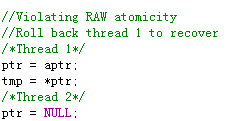
\includegraphics[width=\textwidth]{body/RAW.png}
\caption{RAW atomic violation}
\label {RAW}
\end{minipage}%
\begin{minipage}[t]{0.52\linewidth}
\centering
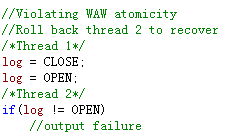
\includegraphics[width=\textwidth]{body/WAW.png}
\caption{Violating WAW atomicity}
\label{WAW}
\end{minipage}
\end{figure}

\begin{figure}
\begin{minipage}[t]{0.52\linewidth}
\centering
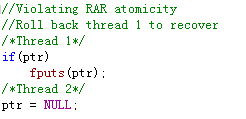
\includegraphics[width=\textwidth]{body/RAR.png}
\caption{RAR atomic violation}
\label {RAR}
\end{minipage}%
\begin{minipage}[t]{0.52\linewidth}
\centering
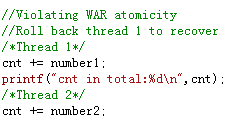
\includegraphics[width=\textwidth]{body/WAR.png}
\caption{Violating WAR atomicity}
\label{WAR}
\end{minipage}
\end{figure}
As in Figure~\ref{RAW}, in thread 1, a global pointer is set to point to aptr and then, dereference it and give the value to a local variable tmp. In thread 2, the global pointer is initialized to NULL. Consider the situation that the first sentence of thread 1 is executed and then thread 2 is executed. When ptr is dereferenced and give its value to tmp, segamentation fault happens. In this case, roll back thread 1 until thread 2 finishes and do the given value part. The bug can be fixed.\\
As in Figure~\ref{WAW}, if thread 2 happens before the end of thread 1, error happens. In this case, rolling back thread 2 can fix the bug.\\
As in Figure~\ref{RAR} and Figure~\ref{WAR}, still rolling back one thread can fix the possible concurrency bugs. In general, for atomic violation bugs, rolling back one thread is sufficient to fix them.
\begin{figure}[t]
\centering
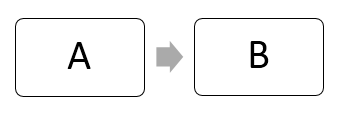
\includegraphics[width=0.7\textwidth]{body/order_violation.png}
\caption{Order violation bug}
\label{order violation}
\end{figure}
\subsection{Recovering order-violation bugs}
Another kind of concurrency bug is called order-violation. That is one thread is required to be finished before another one. For example, in Figure~\ref{order violation}, A is required to finish before B. In this case, roll back B until A finishes can fix the bug.
\subsection{Rocovering deadlock bugs}
A very common concurrency bug in multi-thread programming is deadlock problem. As in Figure~\ref{deadlock}, thread A holds lock 1, thread B holds lock 2 and thread C holds lock 3. A still wants lock 2, while it's held by B. So A is blocked. Similar situation happens in B and C. In this case, roll back any thread can fix deadlock. If roll back B, B releases lock 2, so that C can finish and release lock 3 and 2. Then B can finish. Finally, A can get all resource it wants and finish itself.
\begin{figure}[t]
\centering
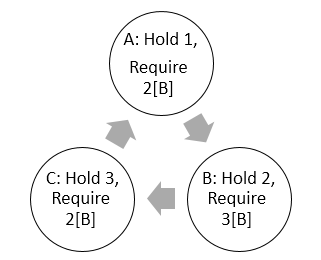
\includegraphics[width=0.7\textwidth]{body/deadlock.png}
\caption{Deadlock}
\label{deadlock}
\end{figure}

\section{Observation II}
For observation II, it indicates that roll back certain area of one thread is sufficient to fix bugs and that area is defined as idempotent region.\\
\textbf{Idempotent region}:a code region that can be reexecuted for any number of times without changing the program semantics.\\
It should end before the failing point because it is meaningless to roll back the error part. Besides it, the idempotent region should not contain any writes to shared variables. If it is, roll back it will continously change a global variable, which is unwanted by users. Furthermore, it will not contain any I/O operations. According to investigation, only 15 \% concurrency bugs contain I/0 operation. In order to guarantee the performance of ConAir, I/O operation is eliminated from idempotent region. Also, it should not contain any writes to local variables that could cause incorrect execution. This rule is also added to guarantee the correnctness of the ConAir. Some local variables, such as static ones is initialized once and changed extends for the entire run of the whole program. If it is included in the idempotent region, potentially incorrect output may happen.\\
All rules are set to guarantee the correctness and performance of the usage of ConAir. Above all, the working principle of the ConAir is to roll back a single thread (failing thread) with its idempotent region.

 